\input{head.inc}

% Präambelbefehle für die Präsentation
\title[TET: Elektrostatik-V: Spiegelungsmethode]{Elektrostatik-V: Spiegelungsmethode}

\begin{document}
% 
% Frontmatter 
% 
%%%%%%%%%%%%%%%%%%%%%%%%%%%%%%%%%%%%%%%%%%%%%%%%%%%%%%%%%%%%%%%%%%%%%%%%%%%%%%%%%%%%%%%%%%%%%%%%%%%%%%%%%%%%%%%%%%%%%%%%%%%%% 

%% inserts the title page and the table of contents
\maketitle

% 
% Content 
% 
%%%%%%%%%%%%%%%%%%%%%%%%%%%%%%%%%%%%%%%%%%%%%%%%%%%%%%%%%%%%%%%%%%%%%%%%%%%%%%%%%%%%%%%%%%%%%%%%%%%%%%%%%%%%%%%%%%%%%%%%%%%%% 
\section{Elektrostatik-V: Spiegelungsmethode}

\begin{frame}

  \frametitle{Idee der Spiegelungsmethode}
  Die \alert{formale Lösung} des Randwertproblems
  \alert{Poisson-Gleichung} mit Randbedingungen \alert{Dirichlet
    und/oder Neumann} im Endlichen mittels \alert{Greenscher Funktionen} hat folgendes aufgezeigt:
  \begin{itemize}[<+->]
    \item Das \alert{Superpositionsprinzip} ist fundamental: Aus einer
      Lösung (Greensche Funktion) der Poisson-Gleichung für eine \alert{Punktladung} ($\delta$-Inhomogenität) folgt formal sofort
      die Lösung für beliebige Inhomogenität $\laddichte{V}(\Ortsr[vs])$: $\phi (\Ortsr[v]) = \int
      G (\Ortsr[v],\Ortsr[vs]) \laddichte{V}(\Ortsr[vs]) \upd^3r'$
      \item Dieser Teil der Lösung ist vollständig durch \alert{die Ladungen
        im Lösungsvolumen} bestimmt
        \item Damit die Gesamtlösung die vorgegeben Randbedingungen
          erfüllt, muss die \alert{Greensche Funktion des Freiraums} $G (\Ortsr[v],\Ortsr[vs]) = \frac{1}{4\pi\varepsilon_0} \frac{1}{|\Ortsr[v]-\Ortsr[vs]|}$ verändert
          werden.
          \item Der zusätzliche Summand ist Lösung der zugehörigen
            \alert{Laplace Gleichung} (homogen, \alert{keine Ladungen
              in V})
              \item \alert{Idee:} Konstruiere für jede Punktladung im
                Lösungsvolumen Ladungen \alert{außerhalb} des
                Lösungsvolumens so, dass in der Überlagerung die
                Randbedingungen erfüllt sind.
                \item Die Ladungen außerhalb haben nur mittelbaren
                  Einfluss auf die Gesamtlösung, indem sie
                  den Einfluss der \alert{influenzieren Oberflächenladungen} nachbilden.
    \end{itemize}

  
  \end{frame}

  \begin{frame}
    \frametitle{Punktladung vor leitender Ebene - Anordnung}
\only<1-2|handout:1>{\resizebox{.8\linewidth}{!}{\begin{tikzpicture}[line width = 1.2pt, line join=round,x=1cm,y=1cm,>=stealth, circuit ee IEC]
	% Fläche
	\draw (0,4) -- (0,-2);
	\draw [decoration=zigzag,decorate] (-0.1,4) -- (-0.1,-2);
        \draw [color=red] (-0.5,3) node[anchor=north] {\circled{2}};
        \draw [color=red] (0.5,3) node[anchor=north] {\circled{1}};
	\draw [->,color=red] (0,3) -- (-1,3) node[anchor=north west] {$\vec{n}$};
	% Erde
	\coordinate (e) at (0,-1.5);
	\draw (e) -- ++(0.7,0) to [ground={pos=1}] (0.7,-2.2);
	\draw (e) circle (1.5pt);
	% Leitfähigkeit, Ladungsdichte
	\draw (-0.1,4) node[anchor=north east] {$\kappa \rightarrow \infty$};
	\draw (0,4) node[anchor=north west] {$\laddichte{F}(x,\,y)=\laddichte{F}(\rho)$};
	% z-Achse
	\draw [->] (0,0) -- (7,0) node[anchor=north west] {$z$};
	% Definitionen für die Punkte
	\coordinate (a) at (4,0);
	\coordinate (b) at (5,3);
	\coordinate (c) at (4,-0.5);
	% Abstand a
	\draw [|<->|] (0,-0.5) -- ++(a);
	\node [label=below:$a$] (X) at ($ (0,-0.5)!.5!(c) $) {};
	% Abstandsvektor
	\draw [->,color=violet] (a) -- (b);
	\draw [color=violet] (4.5,1.5) node[anchor=west]{$\Abstand[v]$};
        \draw [color=violet] (6,1.5) node[anchor=west]{$|\Abstand[v]|=\sqrt{\rho^2+(z-a)^2}$};
	% Ortsvektor
	\draw [->,color=blue] (0,0) -- (b);
	\draw [color=blue] (2.5,1.5) node [anchor=south] {$\Ortsr[v] $};
	% rho
	\draw [|<->|] (5,0) -- (5,3);
	\draw (5,2.5) node[anchor=west] {$\rho$};
        \draw (6,2.5) node[anchor=west] {$\Ortsr[v] = \rho \vu{\rho} + z \vu{z}$}; 
        \draw (6,2) node[anchor=west] {$\Ortsr[vs] =  a \vu{z}= - a \vec{n}$}; 
	% Ladung
	\draw [color=darkgreen] (a) node[anchor=north] {$\ladung$};
	\filldraw [color=darkgreen] (a) circle (1.5pt);
\end{tikzpicture}}}
    \only<2|handout:1>{\vspace{-1.8cm}
      \begin{empheq}[box=\fbox]{align}
          \DFeld{}_2\normal - \DFeld{}_1\normal &= \laddichte{F}\nonumber\\
    \EFeld{}_2\tangential - \EFeld{}_1\tangential & = 0\nonumber
  \end{empheq}}
\only<3|handout:2>{\resizebox{\linewidth}{!}{\usetikzlibrary{calc} 
\begin{tikzpicture}[line width = 1.2pt, line join=round,x=1cm,y=1cm,>=stealth, circuit ee IEC]
	% Leiteroberfläche
	\coordinate (a) at (0,-9);
	\draw (0,4.5) -- ++(a);
	\draw [decoration=zigzag,decorate] (-0.1,4.5) -- ++(a);
	% Raumbezeichnung
	\draw (1.5,4.5) node[anchor=north west] {Lösungsvolumen};
	\draw (-1.5,4.5) node[anchor=north east] {Zusatzvolumen};
	% Koordinaten für Ladung und Spiegelladung
	\coordinate (l) at (6,0);
	\coordinate (sl) at (-6,0);
	% E-Feld um Ladung
	\foreach \l in {0,30,60,90,120,150,180,210,240,270,300,330} \draw [color=red!30!white,->] (l) -- ++(\l:1);
	\draw [color=red] ({6+cos(45)},{sin(45)}) node[anchor=south west] {$\efeld[v]$};
	\coordinate (eu) at (0,{-6*tan(30)});
	\coordinate (eo) at (0,{6*tan(30)});
	\draw [color=red!60!white,dashed] (0,0) -- (7.5,0);
	\draw [color=red!60!white,dashed] (eu) -- (7.5,{1.5*tan(30)});
	\draw [color=red!60!white,dashed] (eo) -- (7.5,{-1.5*tan(30)});
	\coordinate (e) at (1.5,0);
	\coordinate (es) at (1.5,0.15);
	\coordinate (er) at (3,-0.15);
	\draw [color=red,->] (e) -- (0,0);
	\draw [color=red,->] (1,{(6-1)*tan(30)}) -- (eo);
	\draw [color=red,->] (1,{-(6-1)*tan(30)}) -- (eu);
	% E-Feld für Spiegelladung
	% E-Feld um Ladung
	\foreach \l in {0,30,60,90,120,150,180,210,240,270,300,330} \draw [color=blue!30!white,<-] ($(sl) + (\l:0.1)$) -- ++(\l:1);
	\draw [color=blue] ({-6-cos(45)},{sin(45)}) node[anchor=south east] {$\efeld[v]\,'$};
	\draw [color=blue!60!white,dashed] (-7.5,0) -- (0,0);
	\draw [color=blue!60!white,dashed] (eu) -- (-7.5,{1.5*tan(30)});
	\draw [color=blue!60!white,dashed] (eo) -- (-7.5,{-1.5*tan(30)});
	\draw [color=blue,->] (es) -- (0,0.15);
	\draw [color=blue,->] (1,{(6+1)*tan(30)}) -- (eo);
	\draw [color=blue,->] (1,{-(6+1)*tan(30)}) -- (eu);
	% Resultierendes E-Feld
	\draw [color=darkbrown,->] (2,{6*tan(30)}) -- (eo);
	\draw [color=darkbrown,->] (2,{-6*tan(30)}) -- (eu);
	\draw [color=darkbrown,->] (er) -- (0,-0.15);
	\draw [color=darkbrown] (2,{-6*tan(30)}) node[anchor=west] {resultierendes elektrisches Feld};
	% Ladung
	\filldraw [color=darkgreen] (l) circle (1.8pt);
	\draw [color=darkgreen] (l) node[anchor=north] {$\ladung$};
	% virtuelle Ladung
	\filldraw [color=magenta] (sl) circle (1.8pt);
	\draw [color=magenta] (sl) node[anchor=north] {$-\ladung$};
	% Erde eintragen
	\coordinate (erde) at (0,-4.2);
	\draw (erde) -- ++(0.4,0) to [ground={pos=1}] (0.4,-4.7);
	\filldraw (erde) circle (1.5pt);
\end{tikzpicture}}}
\only<4-|handout:3>{\centering{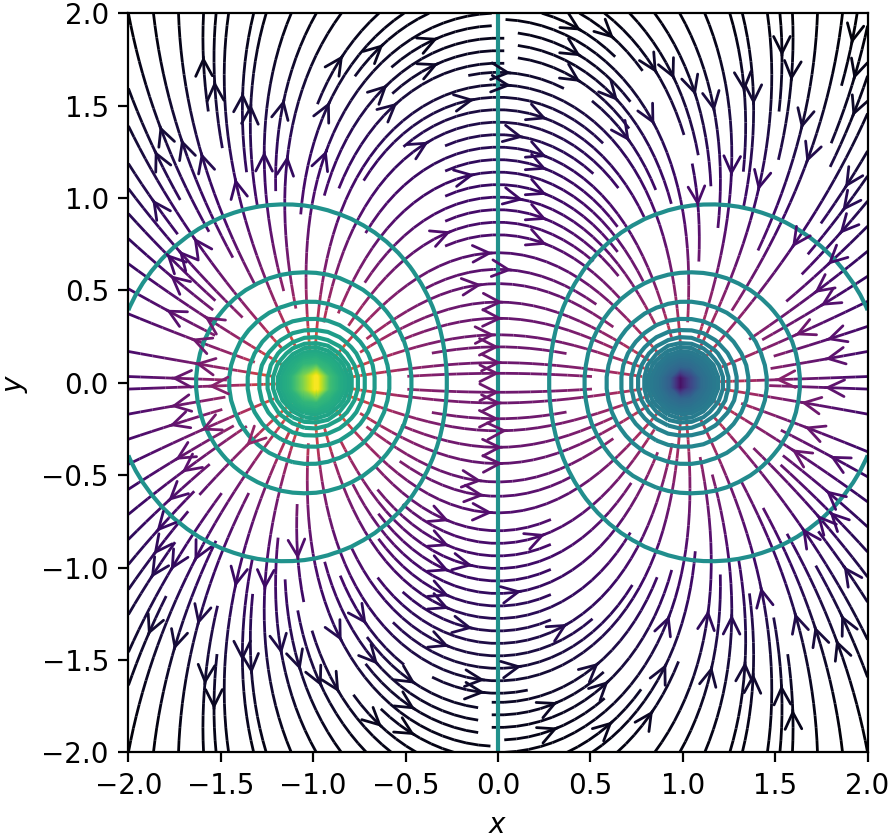
\includegraphics[height=.8\textheight]{programs/dipol.png}}}
\end{frame}

  \begin{frame}
    \frametitle{Berechnung Potential, Feld}

    \begin{itemize}[<+->]
\item  Randbedingungen: \(\EFeld\tangential(z=0) = 0\) bzw. \(\SkalarPot(z=0) = 0\). 

\item Superposition der skalaren Potentiale
  \begin{equation*}
	\SkalarPot(\Ortsr[v]) = \SkalarPot_1 + \SkalarPot_2
		= \durchvierpie \cdot \left[ \dfrac{\ladung}{\sqrt{\rho^2 + (z - a)^2}} + \dfrac{-\ladung}{\sqrt{\rho^2 + (z + a)^2}} \right]
\end{equation*}
\item Da keine Abhängigkeit von \(\varphi\) vorliegt, ergibt sich für das elektrische Feld
\begin{equation*}
	\begin{split}
		\EFeld[v](\Ortsr[v]) = \durchvierpie[\ladung] \cdot
                &\left[ \left( \dfrac{\rho}{\left( \rho^2 + (z - a)^2 \right)^{\nicefrac{3}{2}}} - \dfrac{\rho}{\left( \rho^2 + (z + a)^2 \right)^{\nicefrac{3}{2}}} \right) \cdot \einheitsvek{\uprho} \right. \\
		&	 \left. + \left( \dfrac{z - a}{\left( \rho^2 + (z - a)^2 \right)^{\nicefrac{3}{2}}} - \dfrac{z + a}{\left( \rho^2 + (z + a)^2 \right)^{\nicefrac{3}{2}}} \right) \cdot \einheitsvek{z} \right]
	\end{split}
\end{equation*}
\item Für die Ebene \(z = 0\) gilt demnach
\begin{align*}
	\EFeld[v](z=0) &= \durchvierpie[\ladung] \cdot \left[ 0 \cdot \einheitsvek{\uprho} - 2 \cdot \dfrac{a}{\left( \rho^2 + a^2 \right)^{\nicefrac{3}{2}}} \cdot \einheitsvek{z} \right] \\
		&= -\durchzweipie[\ladung] \cdot \dfrac{a}{\left( \rho^2 + a^2 \right)^{\nicefrac{3}{2}}} \cdot \einheitsvek{z} \\
		&= \EFeld_z \cdot \einheitsvek{z} = -\EFeld\normal \cdot \einheitsvek{z} \pointspacek \to \text{ Nur eine Normalkomponente}
\end{align*}
\end{itemize}
\end{frame}

  \begin{frame}
    \frametitle{Berechnung Ladung}

    \begin{itemize}[<+->]
 \item Stetigkeitsbedingung:  $- \varepsilon_0\EFeld\normal = \varepsilon_0\EFeld_z = \laddichte{F}$ $\to$
\begin{equation*}
	\laddichte{F}(\rho) = -\dfrac{\ladung a}{2 \uppi  \left( \rho^2 + a^2 \right)^{\nicefrac{3}{2}}}
\end{equation*}
\item Gesamtladung der Fläche:
\begin{equation*}
	\ladung_\mathrm{ges. Fläche} = \int\limits_{\varphi'=0}^{2 \uppi} \int\limits_{\rho'=0}^{\infty} \laddichte{F}(\rho') \rho' \intnach{\rho'} \intnach{\varphi'} = -\ladung 
      \end{equation*}
      \item Gesamtladung der Anordnung $=0$ $\to$ Kein Monopolterm in Multipolentwicklung (reiner Dipol!)
\item Zu beachten ist, dass die Gleichungen nur für das Lösungsgebiet gültig sind!
\end{itemize}
\end{frame}

\begin{frame}
\frametitle{Greensche Funktion des Halbraums} $z \ge 0$
\begin{itemize}[<+->]
\item Für die beschriebene Geometrie haben wir das Skalarpotential für
  eine Punktladung gefunden
    \begin{equation*}
	\SkalarPot(\Ortsr[v]) = \SkalarPot_1 + \SkalarPot_2
		= \durchvierpie \cdot \left[
                  \dfrac{\ladung}{\sqrt{\rho^2 + (z - a)^2}} +
                  \dfrac{-\ladung}{\sqrt{\rho^2 + (z + a)^2}} \right]
\end{equation*}
\item Die Punktladung entspricht der $\delta$-Inhomogenität
\item Daher kennen wir nun auch die \alert{Greensche-Funktion des
    Halbraums}
    \begin{equation*}
	G(\Ortsr[v], \Ortsr[vs]) = \durchvierpie \cdot \left[
                  \dfrac{1}{|\Ortsr[v] - \Ortsr[vs]|} -
                  \dfrac{1}{|\Ortsr[v] -\Ortsr[vss]|}
                \right], \quad \Ortsr[vs] = \rho \einheitsvek{\rho} + z \einheitsvek{z} \to \Ortsr[vss] = \rho \einheitsvek{\rho} - z \einheitsvek{z}
              \end{equation*}
            \item Damit können auch \alert{andere Randwertprobleme gleicher Geometrie} gelöst werden:
                     $$
\boxed{      \phi(\Ortsr[v]) = \int_V
  \laddichte{V}(\Ortsr[vs]) G(\Ortsr[v],\Ortsr[vs]) \upd^3\Ortsr[s] + \varepsilon_0 \oint_{O(V)} \left[ G(\Ortsr[v],\Ortsr[vs]) \frac{\partial\phi}{\partial n'} - \phi \frac{\partial G(\Ortsr[v],\Ortsr[vs])}{\partial n'}\right] \upd^2r'}
 $$
 $$
 \frac{\partial G(\Ortsr[v],\Ortsr[vs])}{\partial n'} = \durchvierpie \cdot \left[
                  \dfrac{\Ortsr[v] - \Ortsr[vs]}{|\Ortsr[v] - \Ortsr[vs]|^3} +
                  \dfrac{\Ortsr[v] + \Ortsr[vs]}{|\Ortsr[v] + \Ortsr[vs]|^3}
                \right]\cdot\vec{n}
 $$
  \end{itemize}
\end{frame}

\begin{frame}
\frametitle{Nachrechnen für $\phi(z=0) = \phi_0$}
\begin{itemize}[<+->]
\item Wir gegen wieder in die explizite Form in Zylinderkoordinaten
    \begin{equation*}
	G(\Ortsr[v], \Ortsr[vs]) = \durchvierpie \cdot \left[
                  \dfrac{1}{\sqrt{\rho^2 + (z - a)^2}} +
                  \dfrac{-1}{\sqrt{\rho^2 + (z + a)^2}} \right]
              \end{equation*}
 \item Allgemein:
                     $$
\boxed{      \phi(\Ortsr[v]) = \int_V
  \laddichte{V}(\Ortsr[vs]) G(\Ortsr[v],\Ortsr[vs]) \upd^3\Ortsr[s] + \varepsilon_0 \oint_{O(V)} \left[ G(\Ortsr[v],\Ortsr[vs]) \frac{\partial\phi}{\partial n'} - \phi \frac{\partial G(\Ortsr[v],\Ortsr[vs])}{\partial n'}\right] \upd^2r'}
 $$
\item Für die Normalenableitung am Ort der Oberfläche:
  \begin{align*}
    \left. \frac{\partial G}{\partial n}\right|_{O(V)} & =\left. \gradient G \cdot \vec{n}\right|_{O(V)} = - \left. \frac{\partial G}{\partial z}\right|_{z=0}\\
                                                       &= - \durchvierpie \left[  -\frac{1}{2} ( \rho^2 + (z-a)^2 )^{-\nicefrac{3}{2}}(2z-2a) +\frac{1}{2} ( \rho^2 + (z+a)^2 )^{-\nicefrac{3}{2}}(2z+2a) \right]_{z=0}\\
    &= - \durchvierpie \left[  \frac{a}{(\rho^2 + a^2 )^{\nicefrac{3}{2}}}  + \frac{a}{(\rho^2 + a^2 )^{\nicefrac{3}{2}}} \right] = - \frac{1}{2\pi\varepsilon_0} \frac{a}{(\rho^2 + a^2 )^{\nicefrac{3}{2}}}
  \end{align*}
  \end{itemize}
\end{frame}

\begin{frame}
\frametitle{Nachrechnen für $\phi(z=0) = \phi_0$ (fortgesetzt)}
\begin{itemize}[<+->]
 \item Für Dirichlet Randbedingungen $\phi(z=0) = \phi_0$:
$$
\phi(\Ortsr[v]) = \textcolor{green}{\phi_V} + \textcolor{red}{\phi_{O(V)}} = \textcolor{green}{\int_V
  \laddichte{V}(\Ortsr[vs]) G(\Ortsr[v],\Ortsr[vs]) \upd^3\Ortsr[s]} \textcolor{red}{- \varepsilon_0 \oint_{O(V)} \phi \frac{\partial G(\Ortsr[v],\Ortsr[vs])}{\partial n'} \upd^2r'}
$$
\item Einsetzen der Normalenableitung und des Potentials auf der Oberfläche:
  \begin{align*}
\phi_{O(V)} &= -\varepsilon_0\phi_0 \int_{O(V)} \frac{-1}{2\pi\varepsilon_0} \frac{a}{(\rho^2 + a^2 )^{\nicefrac{3}{2}}} \rho\upd\rho\upd\varphi \\
&=  \phi_0 \int_0^\infty  \frac{a\rho}{(\rho^2 + a^2 )^{\nicefrac{3}{2}}} \upd\rho, \quad \zeta = \rho^2+a^2, \quad \upd \zeta = 2\rho\upd \rho \\ 
            & = \frac{1}{2} \phi_0 a \int_{a^2}^\infty \frac{1}{\zeta^{\nicefrac{3}{2}}} \upd\zeta =  \frac{1}{2} \phi_0 a  \left[ \frac{-2}{\sqrt{\zeta}}  \right]_{a^2}^{\infty} =  \frac{1}{2} \phi_0 a  \left[ -0 + \frac{2}{a}  \right] \\
    &=  \phi_0  \frac{a}{a} =  \phi_0 
    \end{align*}

    \item Wie erwartet gilt also $\boxed{\phi(\Ortsr[v]) = \textcolor{green}{\phi_V} + \textcolor{red}{\phi_0}}$
  \end{itemize}
  
\end{frame}
  

\begin{frame}
  \frametitle{Spiegelung an der Kugel}

  \begin{columns}
 \begin{column}{.5\linewidth}
  \resizebox{\columnwidth}{!}{\begin{tikzpicture}[line width = 1.2pt, line join=round,x=1cm,y=1cm,>=stealth, circuit ee IEC]
	% Achse
	\draw [->] (-2,0) -- (5,0);
	% Kugel
	\draw (0,0) circle (1.5);
	\filldraw (0,0) circle (1.5pt) node[anchor=north] {$M$};
	% Radius
	\draw [<->] (0,0) -- ({1.5*cos(150)},{1.5*sin(150)});
	\draw ({1.5*cos(150)/2},{1.5*sin(150)/2}) node[anchor=south] {$R$};
	% Erde einzeichnen
	\coordinate (erde) at ({1.5*cos(225)},{1.5*sin(225)});
	\draw (erde) -- ++({0.3*cos(225)},{0.3*sin(225)}) -- ++({0.2*cos(225)},0) to [ground={pos=1}] ({2*cos(225)},{2.2*sin(225)});
	\draw (erde) circle (1.5pt);
	% Koordinaten für die Ladung
	\coordinate (l) at (4,0);
	% Koordinaten für die Spiegelladung
	\coordinate (sl) at (1,0);
	% Koordinaten für Punkt P
	\coordinate (p) at (3,2);
	% Vektoren
	\draw [->,color=red] (l) -- (p);
	\draw [color=red] (3.5,1) node[anchor=west] {$R_1$};
	\draw [->,color=red] (sl) -- (p);
	\draw [color=red] (2.2,1) node[anchor=south east] {$R_2$};
	% Strecken
	\draw [|<->|] (0,-1.8) -- (1,-1.8);
	\draw (0.5,-1.8) node[anchor=north] {$s_2$};
	\draw [|<->|] (0,-2.5) -- (4,-2.5);
	\draw (2,-2.5) node[anchor=north] {$s_1$};
	% Ladung
	\filldraw (l) circle (1.5pt) node[anchor=north] {$\ladung$};
	% Spiegelladung
	\filldraw (sl) circle (1.5pt) node[anchor=north] {$-\alpha \ladung$};
	% Punkt P
	\filldraw (p) circle (1.5pt) node[anchor=south] {$\punkt$};
\end{tikzpicture}}
  \end{column}
\begin{column}{.5\linewidth}
  \begin{itemize}[<+->]
  \item Potential
    $$
    \phi(\Ortsr[v]) = \durchvierpie \left[ \frac{Q}{|r\vu{r}-s_1\vu{r}'|}  - \frac{\alpha Q}{|r\vu{r}-s_2\vu{r}'|}   \right]
    $$
  \item Einsetzen von $\phi(\Ortsr[v] = R\vu{r})= 0$:
    $$
     \frac{1}{|R\vu{r}-s_1\vu{r}'|}  = \frac{\alpha }{|R\vu{r}-s_2\vu{r}'|}
     $$
   \item Die Bedingung wird erfüllt mit
     $$
     \boxed{s_2 = \frac{R^2}{s_1}, \quad \alpha = \frac{R}{s_1}}
     $$
    \end{itemize}
  \end{column}
\end{columns}
  \end{frame}


  \begin{frame}
    \frametitle{Greensfunktion der Kugel}
    \begin{itemize}[<+->]
    \item Mit den gefundenen Bedingungen ergibt sich das Potential $\phi$ bzw. die \alert{Greensche Funktion der Kugel} $G(\Ortsr[v],\Ortsr[vs]) = \phi/Q$ zu:
      \begin{align*}
        G(\Ortsr[v],\Ortsr[vs]) & = \durchvierpie \left[ \frac{1}{|\Ortsr[v] - \Ortsr[vs]|}  -  \frac{1}{|\frac{r'}{R}\Ortsr[v] - \frac{R}{r'}\Ortsr[vs]|} \right] \\
        & = \durchvierpie \left[  ( r^2+{r'}^2-2rr'\vu{r}\cdot \vu{r'})^{-\nicefrac{1}{2}}   - \left( \frac{r^2{r'}^2}{R^2}+R^2-2rr'\vu{r}\cdot \vu{r'}  \right)^{-\nicefrac{1}{2}} \right]
      \end{align*}
    \item Symmetrisch, Randbedingung des Potentials erfüllt, Poissongleichung im Lösungsvolumen erfüllt, Eindeutigkeit der Lösung $\to$ fertig!
      \item Wieder kann hiermit eine ganze Klasse von Problem gelöst werden:
                     $$
\boxed{      \phi(\Ortsr[v]) = \int_V
  \laddichte{V}(\Ortsr[vs]) G(\Ortsr[v],\Ortsr[vs]) \upd^3\Ortsr[s] + \varepsilon_0 \oint_{O(V)} \left[ G(\Ortsr[v],\Ortsr[vs]) \frac{\partial\phi}{\partial n'} - \phi \frac{\partial G(\Ortsr[v],\Ortsr[vs])}{\partial n'}\right] \upd^2r'}
 $$
 $$
 \left. \frac{ \partial G(\Ortsr[v],\Ortsr[vs]) }{ \partial n' } \right|_{O(V)} =  - \left. \frac{ \partial G(\Ortsr[v],\Ortsr[vs]) }{ \partial r' }\right|_{r'=R}  = - \durchvierpie \frac{1}{R} \frac{ r^2-R^2 }{ (r^2+R^2-2rR \vu{r}\cdot \vu{r'})^{\nicefrac{3}{2}} }
 $$
      \end{itemize}
  \end{frame}

\begin{frame}
  \frametitle{Mehrere Spiegelebenen}

\begin{itemize}[<+->]
\item Der Fall mehrerer (ideal leitender) Ränder führt zu einer Reihe von Spiegelungen.
\item Hierbei müssen auch die \alert{Spiegelungen der Spiegelung} berücksichtigt werden.
\item Nur bei günstigen Geometrien konvergiert die Reihe.
\end{itemize}
\vspace{1em}

\resizebox{\linewidth}{!}{\begin{tikzpicture}[scale=0.8, line width = 1.2pt, line join=round,x=1cm,y=1cm,>=stealth, circuit ee IEC]
	% Koordinaten für die Spiegelfläche
	\coordinate (a) at (0,2);
	\coordinate (b) at (0,-4);
	\coordinate (c) at (4,2);
	% Ladungsdichten 1. Spiegelung
        \onslide<4->{
	\draw (3.5,0) node[anchor=east] {$\laddichte{V}$};
	\draw (3.5,0.75) -- (2,0) -- (3.5,-0.75) -- cycle;}
      \onslide<5->{
	\draw (-3.5,0) node[anchor=west] {$-\laddichte{V}$};
	\draw (-3.5,0.75) -- (-2,0) -- (-3.5,-0.75) -- cycle;}
      \onslide<6->{
	\draw (4.5,0) node[anchor=west] {$-\laddichte{V}$};
	\draw (4.5,0.75) -- (6,0) -- (4.5,-0.75) -- cycle;}
      % Ladungsdichten 2. Spiegelung
      \onslide<7->{
	\draw [color=red] (-4,2) -- ++(b);
	\draw [color=red] ({3.5-8},0) node[anchor=east] {$\laddichte{V}$};
	\draw [color=red] ({3.5-8},0.75) -- ({2-8},0) -- ({3.5-8},-0.75) -- cycle;}
      \onslide<8->{
	\draw [color=red] ({3.5+8},0) node[anchor=east] {$\laddichte{V}$};
	\draw [color=red] (8,2) -- ++(b);
	\draw [color=red] ({3.5+8},0.75) -- ({2+8},0) -- ({3.5+8},-0.75) -- cycle;}
      % Spiegelflächen
      \onslide<4->{
	\draw (a) -- ++(b);
	\draw[decoration=zigzag,decorate] (-0.15,2) -- ++(b);
	\draw (c) -- ++(b);
	\draw[decoration=zigzag,decorate] (4.15,2) -- ++(b);
	% Erdung
	\coordinate (erde) at (0,-1.5);
	\draw (erde) -- ++(0.4,0) to [ground={pos=1}] (0.4,-1.9);
	\filldraw (erde) circle (1.5pt);
	\coordinate (erdez) at (4,-1.5);
	\draw (erdez) -- ++(-0.4,0) to [ground={pos=1}] (3.6,-1.9);
	\filldraw (erdez) circle (1.5pt);}
\end{tikzpicture}}

\end{frame}
  
\input{finalframe.inc}
   
\end{document}